\documentclass[a4paper,11pt]{article}
\usepackage[dutch]{babel}
\usepackage[pdftex]{graphicx}
\pagestyle{plain}
\title{Verslag Project}
\author{Mathy Vanhoef \and Robin Timmermans}
\begin{document}

\maketitle

\section{Taakverdeling}

Mathy:

\begin{itemize}
\item Volledige Grafische User Interface (behalve QDialogBoekInfo)
\end{itemize}

\noindent Robin:

\begin{itemize}
\item Interne voorstelling van het boek
\item Xml reader en writer
\end{itemize}

\noindent In de headers van de klassen staat wie deze klasse heeft geschreven.

\section{Klassediagram}

De interne voorstelling van een Boek is duidelijk zichtbaar in het UML diagram. Bij de interne voorstelling zijn verschillende
dingen veranderd:

\begin{itemize}
\item Verschillende member variablen die vroeger in Boek zaten, hebben we nu in BoekInformatie geplaats. Voorbeelden
zijn de titel, auteurs en versie.
\item In de abstracte Component klasse hebben we een nieuwe pure virtuele functie toegevoegd. Deze functie, SetDefault,
geef de component een default inhoud (de tekst, foto, enz.). Zie hiervoor ook de code om van een pagina een layout te maken!
\item Een tweede pure virtuele functie die we aan Component hebben toegevoegd is toXml.
\item Bij Pagina en Deel hebben we ook ``move up'' en ``move down'' functies toegevoegd. In Deel werken deze functies in
op de volgorde van de pagina's, en bij Pagina op de volgorde van de Componenten.
\end{itemize}

Het grootste nieuwe deel zijn alle klassen die worden gebruikt voor de GUI. In het UML schema kan dat een beetje verwarrend
zijn omdat sommige klassen geen duidelijke verbindingen hebben (zoals de vele dialogen die worden gebruikt). De belangrijkste
klasse is de MainWindow, die het hoofdvenster weergeeft. De drie belangrijkste widgets die in het hoofdvenster worden
getoond zijn ComponentManager, HierarchieManager en Editor. Het MainWindow bepaald waar deze widgets komen te staan.
Het bevat ook een ProjectManager die de drie widgets (ComponentManager, HierarchieManager en Editor) met elkaar
verbindt en beheert.

Het widget Editor bevat ComponentList en PubGraphicsScene. De scene geeft alle klassen afgeleid van QGraphicsItem weer.
Al deze klassen (afgeleid van QGraphicsItem) die een component in de scene voorstellen, erven ook van de ``interface''
IQGraphicsComp. Deze interface heeft bijvoorbeeld een pure virtuele functie openEditDialog die een dialoog toont om de
eigenschappen van het component te veranderen. Elk component heeft dus ook een dialoog, welk in een aparte klasse staat.

Verder is er nog een Opties klasse en een LayoutManager klasse die alletwee ook verschillende dialogen gebruikt. Deze dialogen
zijn ook weer in aparte klassen gemaakt.

\section{Algoritmes en Datastructuren}

Het project bevat weinig complexe algoritmes. Het zijn vooral de onderlinge verbindingen van klassen die soms ingewikkeld
kunnen worden, maar hiervoor hebben we het UML schema!

De datastructuur die we het meest hebben gebruikt in de onderliggende voorstelling van een Boek is de list klasse uit de
standaard template library van C++. Dit omdat een boek vele delen kan bezitten, en een deel op zijn beurd vele pagina's
kan bezitten. Hiervoor is een gelinkte lijst ideaal, en dit gebruikt list onderliggend.

Behalve bij de lijst van autuers hebben we niet list, maar vector gekozen. Dit omdat er meestal maar tussen de 1 of 4
auteurs van een boek zijn. Er zullen dus relatief weinig element in worden opgeslagen waardoor een vector in
dit geval beter is.

\section{Handleiding}

\subsection{Opbouw van een Boek}

Een boek bevat verschillende delen. Meestal zullen deze delen een hoofdstuk voorstellen. Elk van deze delen bevat op zijn
beurt een lijst van pagina's. Een pagina bestaat tenslotte uit een lijst van componenten. Verder kan je ook de nodige
informatie van het boek instellen (auteurs, ISBN, etc.)

\subsection{Beginnen}

Om te kunnen beginnen moet je eerst een nieuw boek maken of een bestaand boek openen, want anders zijn alle widgets gedisabled.

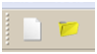
\includegraphics{fig1.png}

Als je een file hebt geopend kun je het boek gewoon aanpassen. Als je een nieuw file hebt gemaakt moet je eerst een deel toevoegen.

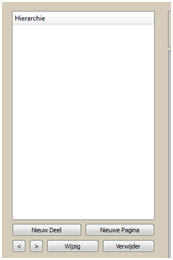
\includegraphics{fig2.png}

Daarna moet je het deel selecteren en een pagina  toevoegen.

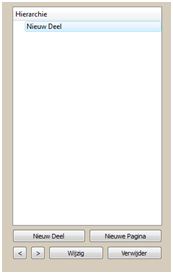
\includegraphics{fig3.png}

Nu moet je op de pagina dubbelklikken zodat de grote kader rechts (de editor) wit wordt en kan je van boven elementen
naar de editor eronder slepen.

\subsection{Pagina Bewerken}

Je kan elementen van boven naar de pagina eronder slepen.


\includegraphics{fig4.png}

Als je een component wilt veranderen kan je er op dubbelklikken zodat er een dialog te voorschijn komt waar je de eigenschappen kunt aanpassen.
Een component kan verplaatst worden door te slepen. Je kan een component  resizen door rechtsonder te gaan zodat het muisicoon verandert in de
gebruikelijke dubbele pijl. Je kan ook het element linksonder in het kader selecteren en dan op wijzig klikken.

\subsection{Layout}

Als je van een pagina een layout wilt maken klik je in het menu op layout, nieuwe layout. Als je een layout wilt veranderen maak je eerst een pagina
aan gebasseerd op de layout die je wilt wijzigen, verander je de pagina, en daarna maak je er een nieuwe layout van.

\subsection{Boek Informatie}

Bij het aanmaken van een boek komt een dialoog tevoorschijn waar je de boekinformatie kunt aanpassen. Wil je ze daarna nog aanpassen dan moet je
op tools, boekinformatie klikken zodat je hetzelfde dialoog krijgt.

\subsection{Openen en Opslaan}

Om een boek op te slaan klik je op file, open of file, save in het menu. Je kan ook de knoppen op het hoofdscherm gebruiken of de shortkey's
CTRL+O en CTRL+S.

\end{document}
